% paper format, language, badness tolerance, document class
%\documentclass[a4paper,twocolumn]{article}
%\hbadness 1107  %twocolumn -> badness ?!
%\vbadness 1776
%\documentclass[a4paper]{article}
%\documentclass[a4paper,ngerman]{article}
%\documentclass[a4paper,ngerman,twocolumn]{article}
%\documentclass[a6paper,ngerman,twocolumn]{book}
% obiges a6paper wird nicht genommen -> geometry Paket mit a6paper
\documentclass[ngerman,10pt]{book}
%\documentclass[ngerman,10pt]{extbook}
%\usepackage[cm]{fullpage}
%\usepackage[top=tlength, bottom=blength, left=llength, right=rlength]{geometry}
\usepackage[a5paper]{geometry}
\geometry{hmargin={2cm,1.5cm},vmargin={1.5cm,1.5cm}}
%\special{papersize=210mm,297mm}

% source code character set
%\usepackage[utf8]{inputenc}
%\usepackage[ansinew]{inputenc}

% word wrap correctly for German
%\RequirePackage{hyphsubst}
%\HyphSubstIfExists{ngerman-x-latest}{\HyphSubstLet{ngerman}{ngerman-x-latest}}{}
%\listfiles
%\usepackage{babel}
\RequirePackage[ngerman=ngerman-x-latest]{hyphsubst}
\usepackage{babel}
\usepackage{ziffer}
%\usepackage[babel,german=quotes]{csquotes}
%\usepackage[babel,german=guillemets]{csquotes}
\usepackage[babel]{csquotes}
\DeclareQuoteStyle[typo]{german}
    {\glqq}{\grqq}  %aussen
    {\glq}{\grq}    %innen
\setquotestyle[typo]{german}

% enumerations
%   http://texblog.org/2008/10/16/lists-enumerate-itemize-description-and-how-to-change-them/
%   https://en.wikibooks.org/wiki/LaTeX/List_Structures#Customizing_enumerated_lists
%\renewcommand{\theenumi}{\arabic{enumi}}
%\renewcommand{\labelenumi}{\theenumi.)}
%\usepackage{enumerate}
\usepackage{paralist}
%   http://rtm.wustl.edu/writings/htfasttex.pdf
%   http://de.wikibooks.org/wiki/LaTeX-W%C3%B6rterbuch:_newenvironment
% -- Einrückung von itemize und enumerate gleich
%   http://tex.stackexchange.com/questions/97305/how-to-change-the-indentation-of-all-enumerates
\setdefaultleftmargin{0cm}{}{}{}{}{}
% -- Nummerierung vor enumerate
\setdefaultenum{1.)}{}{}{}
% -- Nummerierung vor itemize
%\def\buolist{\begin{enumerate}[1)]}
%\def\euolist{\end{enumerate}}
%\def\bolist{\begin{enumerate}[1.)]}
%\def\eolist{\end{enumerate}}
%\newenvironment{uolist}[0]  % easier to extend, but need to type \begin{uolist}
%    {\begin{enumerate}[1)]}
%    {\end{enumerate}}
%\newenvironment{olist}[0]
%    {\begin{enumerate}[1.)]}
%    {\end{enumerate}}
\renewenvironment{itemize}[0]
    {\begin{enumerate}[1)]}
    {\end{enumerate}}

% table of contents
%   http://www.ctan.org/pkg/tocloft
\setcounter{tocdepth}{2}    %default: 3
\usepackage[titles]{tocloft}
\setlength{\cftbeforesecskip}{0ex}
\setlength{\cftsecindent}{0em}
\setlength{\cftsubsecindent}{1em}
% Abstände zwischen Einträgen
\renewcommand\cftchapafterpnum{\vskip1mm}
%\renewcommand\cftsecafterpnum{\vskip0pt}

% headlines
% no numbering
%   sec 4.2 @ http://mirrors.ctan.org/macros/latex/contrib/titlesec/titlesec.pdf
\setcounter{secnumdepth}{-1} % = nur Teile werden nummeriert

% code listing
\usepackage{xcolor}
\usepackage{listings}
\lstdefinestyle{ShellInput}{
    language=bash,
    deletecomment=[l]\#,
    %basicstyle=\small\ttfamily,
    %basicstyle=\small,
    basicstyle=\bfseries,
    numbers=left,
    numberstyle=\tiny,
    numbersep=3pt,
    frame=tb,
    columns=fullflexible,
    backgroundcolor=\color{yellow!20},
    linewidth=0.9\linewidth,
    xleftmargin=0.1\linewidth
}
\lstset{
    % http://de.wikibooks.org/wiki/LaTeX-W%C3%B6rterbuch:_Schriften
    basicstyle=\upshape\ttfamily\mdseries,
    commentstyle=\itshape\ttfamily\mdseries,
    numbers=left,
    numberstyle=\small\upshape,
    numbersep=8pt,
    frame=single,
    language=Pascal,
    framexleftmargin=15pt,
    breaklines=true
}
\newcommand*{\Package}[1]{\texttt{#1}}%

% font (only for XeTeX and LuaTeX)
\usepackage{fontspec}
%\setmainfont{Droid Sans}   % enthält keine kursive Schrift
\setmonofont{Droid Sans Mono}
%\setmainfont{DejaVu Sans Condensed}
%\setmainfont{DejaVu Sans Extralight}
%\setmonofont{DejaVu Sans Mono}
%\setmainfont{Open Sans}    % enthält keine Monospace Schrift
%\setmainfont{Open Sans Light}
\setmainfont[      % normal = light, fett = normal
    BoldFont={Open Sans},
    ItalicFont={Open Sans Light Italic},
    BoldItalicFont={Open Sans Italic}
    ]{Open Sans Light}
%\setmainfont{Corbel}   %test

% bibliography
\usepackage{natbib}

% figures
\usepackage{graphicx}
% use whole column width by default
\setkeys{Gin}{width=\columnwidth, height=!}

% colored TODOs
\usepackage{color}
\usepackage{xparse}
\NewDocumentCommand{\TODO}{g}{
    \IfNoValueTF{#1}
        { \textcolor{red}{TODO} }
        { \textcolor{orange}{TODO[#1]} }
}

% ISO 8601 Datumsformat
%\usepackage[style=iso]{datetime2}
\usepackage[iso]{datetime}

% Befehle für semantische Auszeichnung
\newcommand*{\Fachbegriff}[1]{\emph{#1}}
\newcommand*{\Code}[1]{\texttt{#1}}

% Abstand zwischen Absätzen
%\setlength{\parskip}{0.20cm}%\baselineskip}
% gut für textastige Dokumente, aber hat Nachteil dass die Einträge im Inhaltsverzeichnis auch Absätze sind. Wenn viele Einträge vorhanden sind kann man den Abstand der Einträge nicht unter der Absatz-Abstand reduzieren.

% Tabelle über mehrere Seiten
\usepackage{longtable}  % geht über mehrere Seiten, aber keine selbst erweiterbaren Spalten
%\usepackage{tabulary}   % gut, aber nicht über mehrere Seiten
%\usepackage{tabularx}   % nicht schlecht, aber nicht über mehrere Seiten
\usepackage{tabu}       % bestes, benötigt longtable
% Handbuch @ http://mirror.easyname.at/ctan/macros/latex/contrib/tabu/tabu.pdf

% Stichwortverzeichnis
%\usepackage{makeidx}
%\renewcommand{\indexname}{Stichwortverzeichnis}
% ^ funktoniert nicht (mehr?)
\usepackage[original]{imakeidx}
% Handbuch @ http://mirror.easyname.at/ctan/macros/latex/contrib/imakeidx/imakeidx.pdf
% Stichwortverzeichnis initialisieren
\makeindex[title=Stichwortverzeichnis,intoc=true]

% hyperlinks
%   en.wikibooks.org/wiki/LaTeX/Hyperlinks
%   http://www.golatex.de/verlinktes-inhaltsverzeichnis-texniccenter-t2281.html
%   -> load as last as it redefines index-related commands
\usepackage[unicode=true,pagebackref=false]{hyperref}
\hypersetup{
    breaklinks=true,
    %bookmarks=true,
    linktoc=all,            % none,section,page,all
    pdfauthor={Die Kontaktberichte-Register-Autoren},
    pdftitle={Kontaktberichte-Register},
    pdfsubject={Thema},
    pdfkeywords={keyword1} {keyword2} {keyword3},
    colorlinks=true,
    urlcolor=blue,          % external links
    linkcolor=black,        % internal links
    linkbordercolor=red,
    citecolor=black,        % links to bibliography
    filecolor=magenta,      % file links
    pdfborder={0 0 0}
}
\urlstyle{same}  %do not use monospace font for urls

% meta information
\title{Kontaktberichte-Register \\ --- \\ \Large{Nummern 1 bis 596}}
\author{Die Autoren des Kontaktberichte-Registers}
%\date{2016-06}
\date{!!DATEN-DATUM!!}%\today}

\begin{document}
\frontmatter



% Titelseite
\maketitle




% linke Seite mit Copyright-Vermerk
\thispagestyle{empty}
\null    % benötigt damit vfill funktioniert
\vfill

\noindent Copyright {\textcopyright} 2016 bis {\the\year} die Autoren des Kontaktberichte-Registers. Die komplette Autorenliste ist im Kapitel \emph{\nameref{ch:mitwirkende}} auf Seite \pageref{ch:mitwirkende} zu finden.%aufgelistet.

\vspace{2mm}

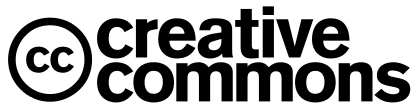
\includegraphics[height=10mm,keepaspectratio=true]{CreativeCommons_logo_trademark}
%
\includegraphics[height=10mm,keepaspectratio=true]{chooser_cc}

\includegraphics[height=10mm,keepaspectratio=true]{chooser_by} 
\includegraphics[height=10mm,keepaspectratio=true]{chooser_nc} 
\includegraphics[height=10mm,keepaspectratio=true]{chooser_nd}

\vspace{2mm}

\noindent Dieses Werk ist lizenziert unter der Creative Commons Namensnennung-Nicht kommerziell 4.0 International Lizenz. Für eine Kopie der Lizenz besuche \url{http://creativecommons.org/licenses/by-nc-nd/4.0/}. Die nicht-"-kommerzielle Verwendung ist daher ohne weitere Genehmigung der Urheber ausdrücklich erlaubt.

\vspace{2mm}

\noindent Projekt-Seite: \url{https://github.com/ERnsTL/kontaktberichte-register}

\vspace{2mm}

\noindent Erzeugt: !!ERZEUGT-DATUM!! \\
Daten-Version: !!DATEN-VERSION!! von !!DATEN-DATUMZEIT!!

\newpage



\chapter*{Abkürzungen}

\begin{description}
	\item[PPK] Plejadisch-plejarische Kontaktberichte (Serie aller Blöcke)
	\item[PPKB] Plejadisch-plejarische Kontaktberichte Block x (ein bestimmter)
	\item[KB] Kontaktbericht
	\item[S] Seite, bezogen auf eine bestimmte Ausgabe
	\item[V] Vers = Satz
	\item[A] Abschnitt
	\item[K] Kapitel
	\item[GL] Geisteslehre
	\item[B] Brief
\end{description}



\chapter*{Abkürzungen}

\begin{description}
\item[PPK] Plejadisch-plejarische Kontaktberichte-Block
\item[KB] Kontaktbericht
\item[S] Seite, bezogen auf eine bestimmte Ausgabe
\item[V] Vers = Satz
\item[A] Abschnitt
\item[K] Kapitel
\item[GL] Geisteslehre
\item[B] Brief
\end{description}



% Inhaltsverzeichnis-Seite
\tableofcontents



\mainmatter

!!BUCH-ANFANG!!
\chapter{!!TITEL!!}

Bezogen auf Ausgabe !!AUSGABE-JAHR!!. Enthält die Kontaktberichte !!KB-VON-NAME!! bis !!KB-BIS-NAME!! aus dem Zeitraum !!KB-VON-DATUM!! bis !!KB-BIS-DATUM!!.



!!KAPITEL-ANFANG!!
\section{KB!!NAME!! von !!DATUM!! !!ZEIT!!}

Personen: !!PERSONEN!!. !!EINLEITUNG!!

\tabulinesep = 1.5mm
\extrarowsep = 0mm
%\begin{longtabu} to \linewidth {rrlX}
\begin{longtabu} to \linewidth {rrrX}


%\rowfont\bfseries V & S & Sprecher & Inhalt \\ \hline
\rowfont\bfseries von & bis & S & Inhalt \\ \hline
\endhead

%\\ \hline
\hline
%\multicolumn{4}{r}{Fortsetzung auf nächster Seite} \\
\endfoot

%\\ \hline
\hline
\endlastfoot

!!EINTRAG-ANFANG!!
%!!SATZ-VON!! & !!SATZ-BIS!! & !!SPRECHER!! & !!INHALT!! \\
!!SATZ-VON!! & !!SATZ-BIS!! & !!SEITE-VON-BIS!! & !!INHALT!! \\
!!EINTRAG-ENDE!!
\end{longtabu}



!!KAPITEL-ENDE!!



!!BUCH-ENDE!!



\chapter*{Mitwirkende}
\addcontentsline{toc}{chapter}{Mitwirkende}
\label{ch:mitwirkende}

Ein herzlicher Dank ergeht an:

\vspace{2mm}

\noindent
!!AUTOREN!! \\



% Stichwörter-Querverweise
\index{Billy, Eduard Albert Meier|seealso{Billy}}
\index{Plejadier|see{Plejaren}}



% Stichwortverzeichnis einfügen
\printindex



\end{document}
